\section{Auswertung}
\label{sec:Auswertung}
Lineare Regression durchgeführt für:
\begin{equation*}
    \ln\left(\frac{U_c}{U_0}\right)=-\frac{1}{RC}\cdot t + b.
\end{equation*}
Es ergibt sich daraus:
\begin{align*}
  RC &= (0.39001\pm 0.00056)\unit{\milli\second}\\
  b &= (0.030872\pm 0.021421).\\
\end{align*}
%(-2564.035208002769, 37.56001783858995, 0.03087285853896417, 0.02142147040602549)
\begin{figure}
  \centering
  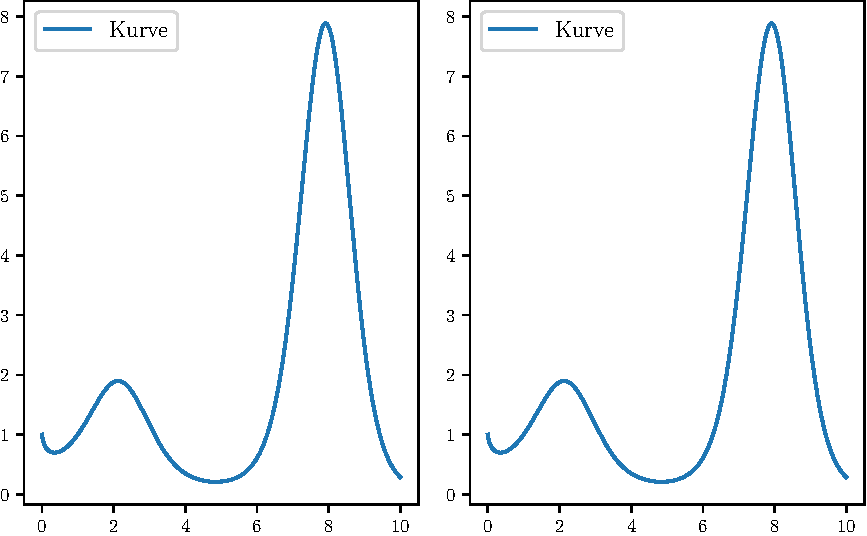
\includegraphics{plot.pdf}
  \caption{Lineare Regression und Messdaten zur Bestimmung der Zeitkonstante RC über den Entladungsprozesses des Kondensators.}
  \label{fig:plot}
\end{figure}

\begin{figure}
  \centering
  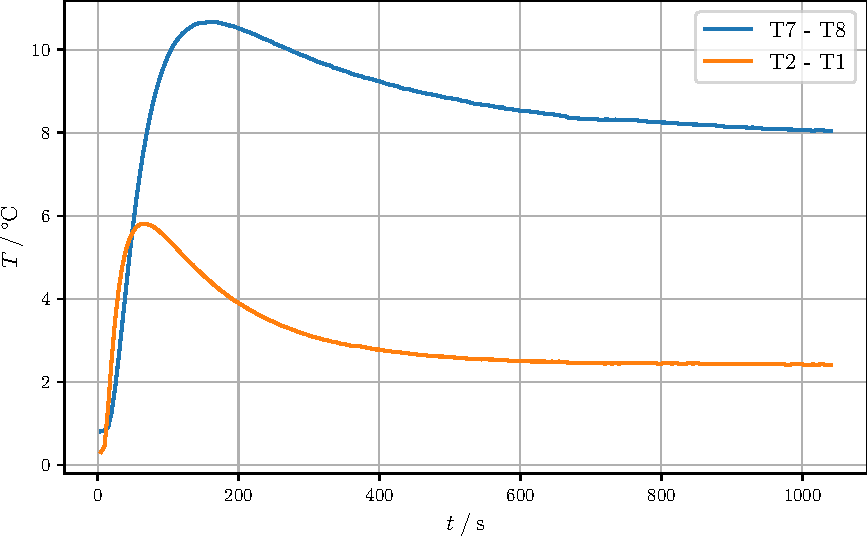
\includegraphics{plot2.pdf}
  \caption{}
  \label{fig:plot2}
\end{figure}
Gefitted an:
\begin{equation*}
  \frac{A(f)}{U_0} = \exp(-a\cdot f + b)
\end{equation*}
Die Parameter sind hier:
\begin{align*}
  a = 2.6401 \unit{\milli\second} = RC
  b = 0.99545
\end{align*}

\begin{figure}
  \centering
  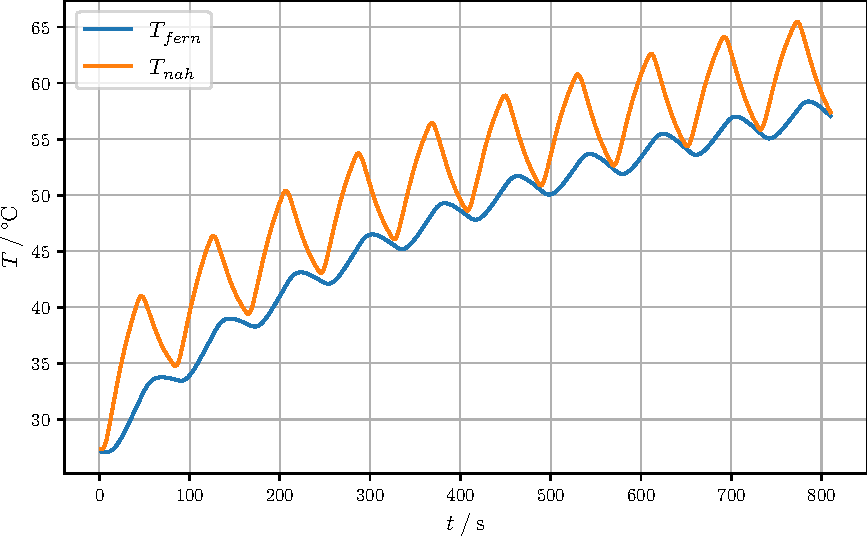
\includegraphics{plot3.pdf}
  \caption{}
  \label{fig:plot3}
\end{figure}
Gefitted an:
\begin{equation*}
  \symup{\phi} = a*\arctan(b*t)
\end{equation*}
Die Parameter hier:
\begin{align*}
  a &=0.9862 \\
  b &=6.9641 \unit{\milli\second} = RC \\
\end{align*}

\begin{figure}
  \centering
  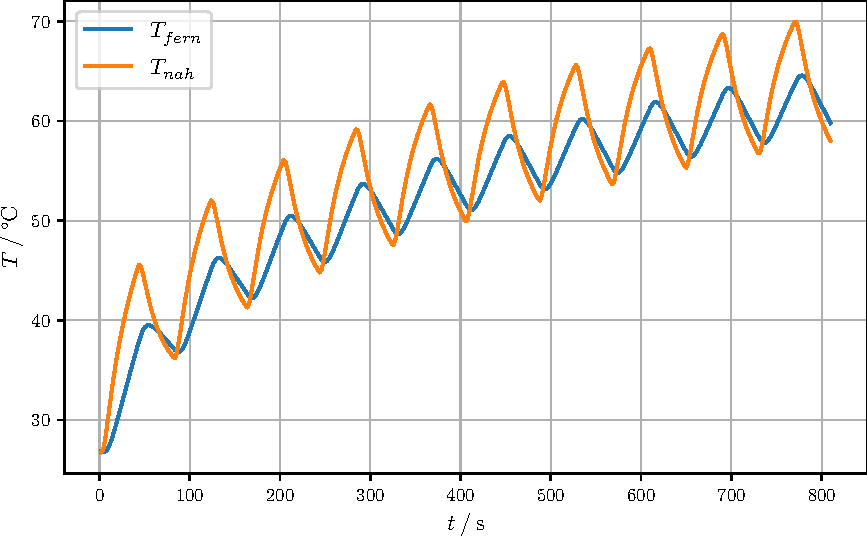
\includegraphics{plot4.pdf}
  \caption{}
  \label{fig:plot4}
\end{figure}

Siehe \autoref{fig:plot}!
